\clearpage
\newpage
\appendix

\section{Training Dynamics}
\label{app:dynamics}
We provide the loss and gradient norm curves for the controlled ablation studies in Section~\ref{subse:ranking_learn} in \Cref{fig:loss_ab}. The training dynamics reveal distinct optimization behaviors across designs. The inner-softmax gate consistently achieves lower training loss than the outer-gate formulation. Independent sigmoid gates and raw-logit injection achieve even lower losses, but fail to improve sparsification, as both effectively approach ungated attention and learn little discriminative block ranking. Similarly, although the STE formulation yields lower training loss, its final sparsification performance remains inferior, indicating that training loss alone is insufficient to assess ranking quality. Hard gating further reduces loss while substantially increasing the gradient norm, suggesting more aggressive optimization. Sparse-scope training starts with higher loss but gradually approaches full-scope training, indicating that the two scopes can eventually reach comparable solutions despite different gradient dynamics. Overall, effective selector training requires not only loss minimization but also preservation of a meaningful and discriminative block ranking signal.

\begin{figure}[h]
    \centering

    \begin{subfigure}{0.99\linewidth}
        \centering
        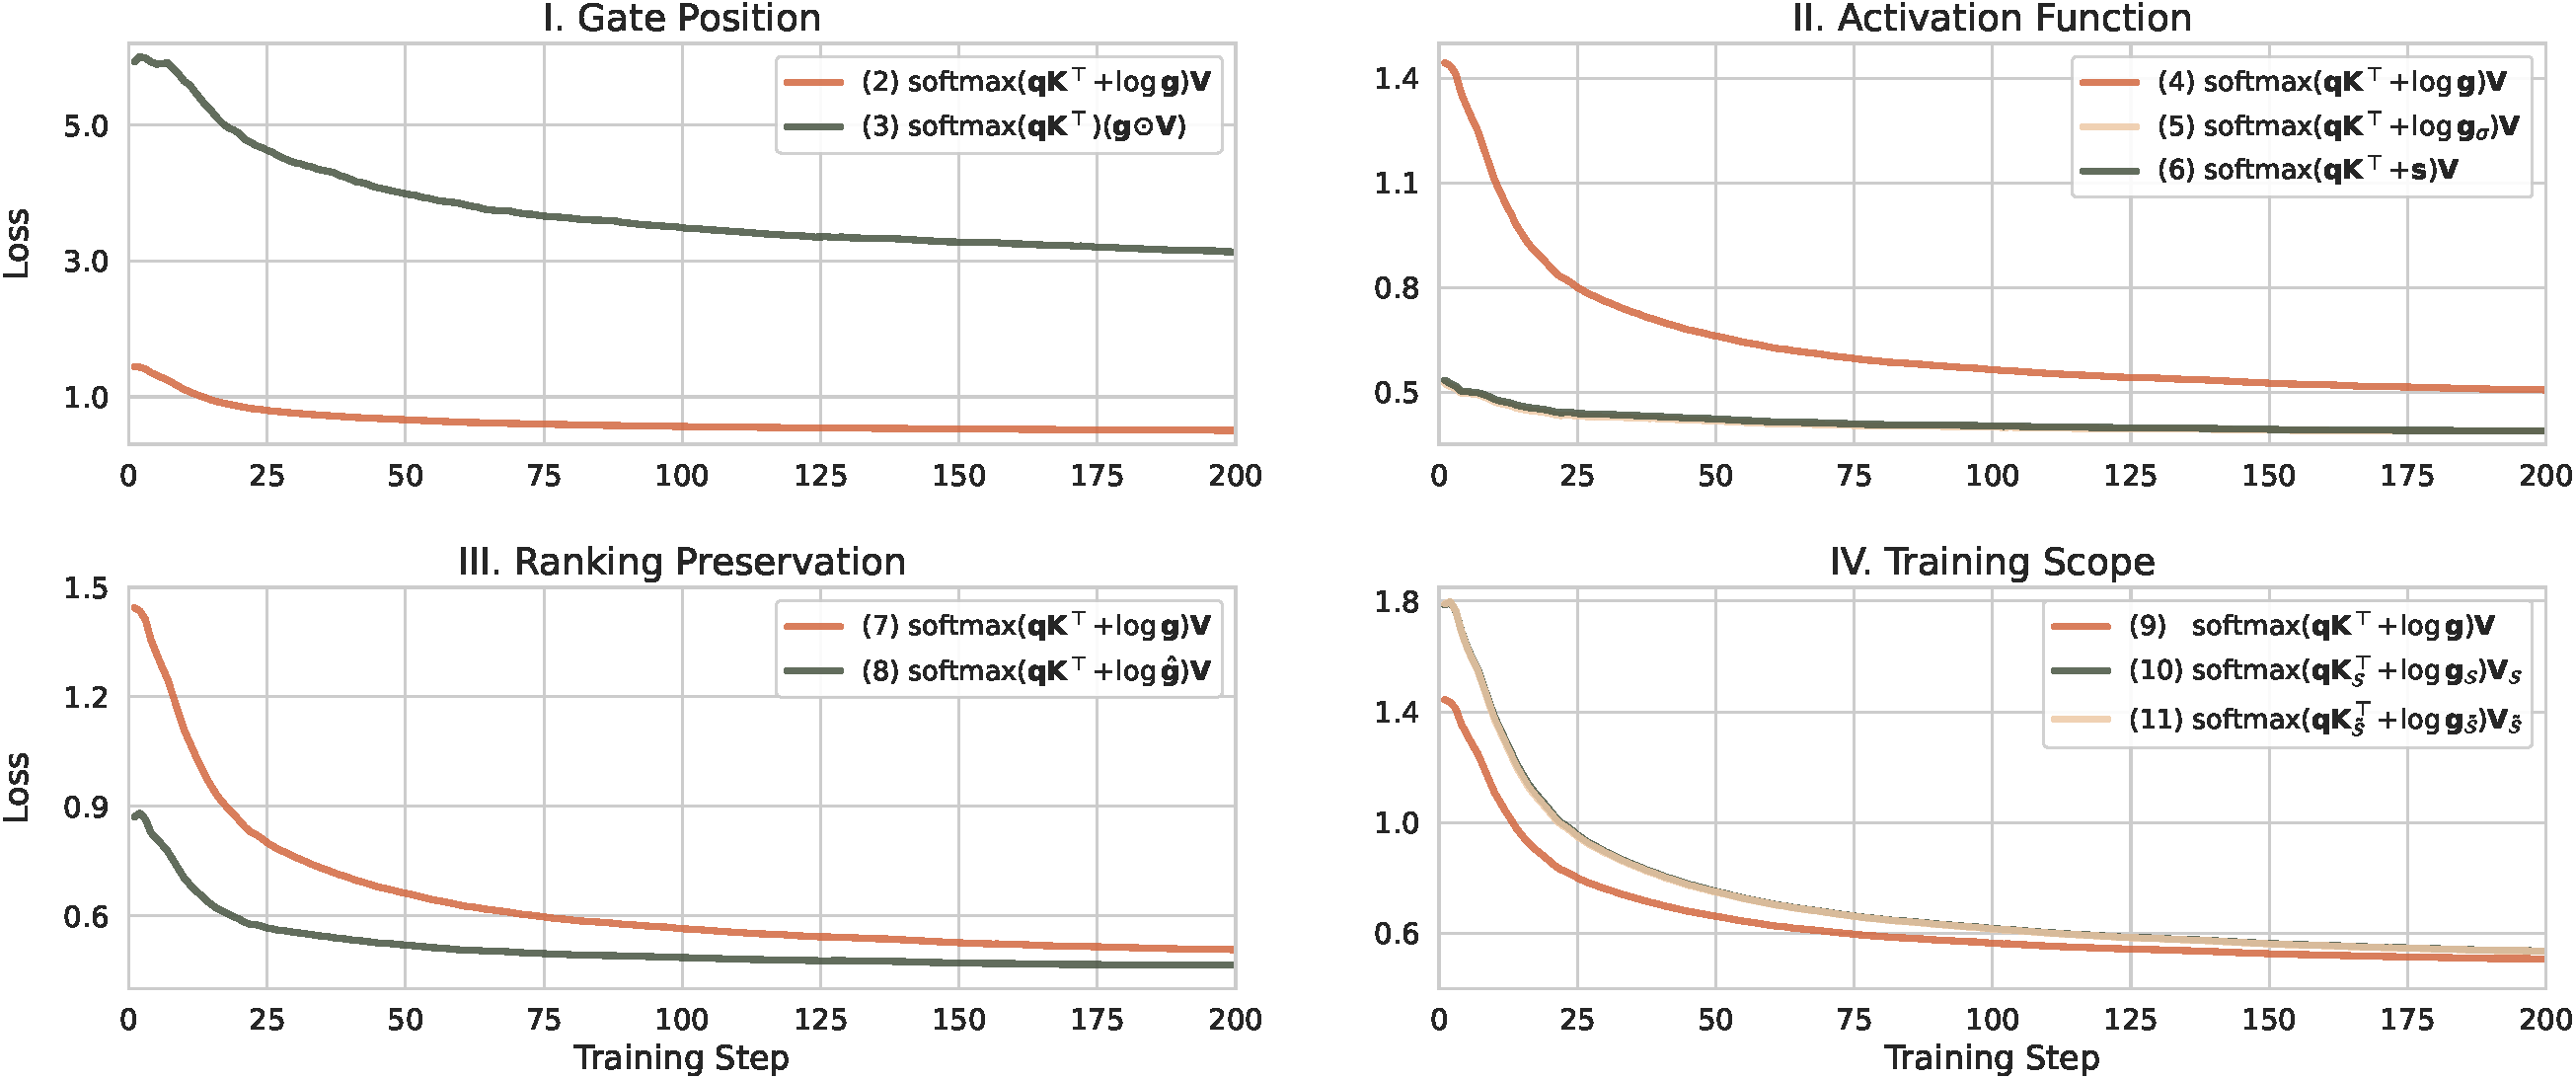
\includegraphics[width=\linewidth]{sec/fig/ablation_loss_curves1.pdf}
        \caption{}
    \end{subfigure}


    \begin{subfigure}{0.99\linewidth}
        \centering
        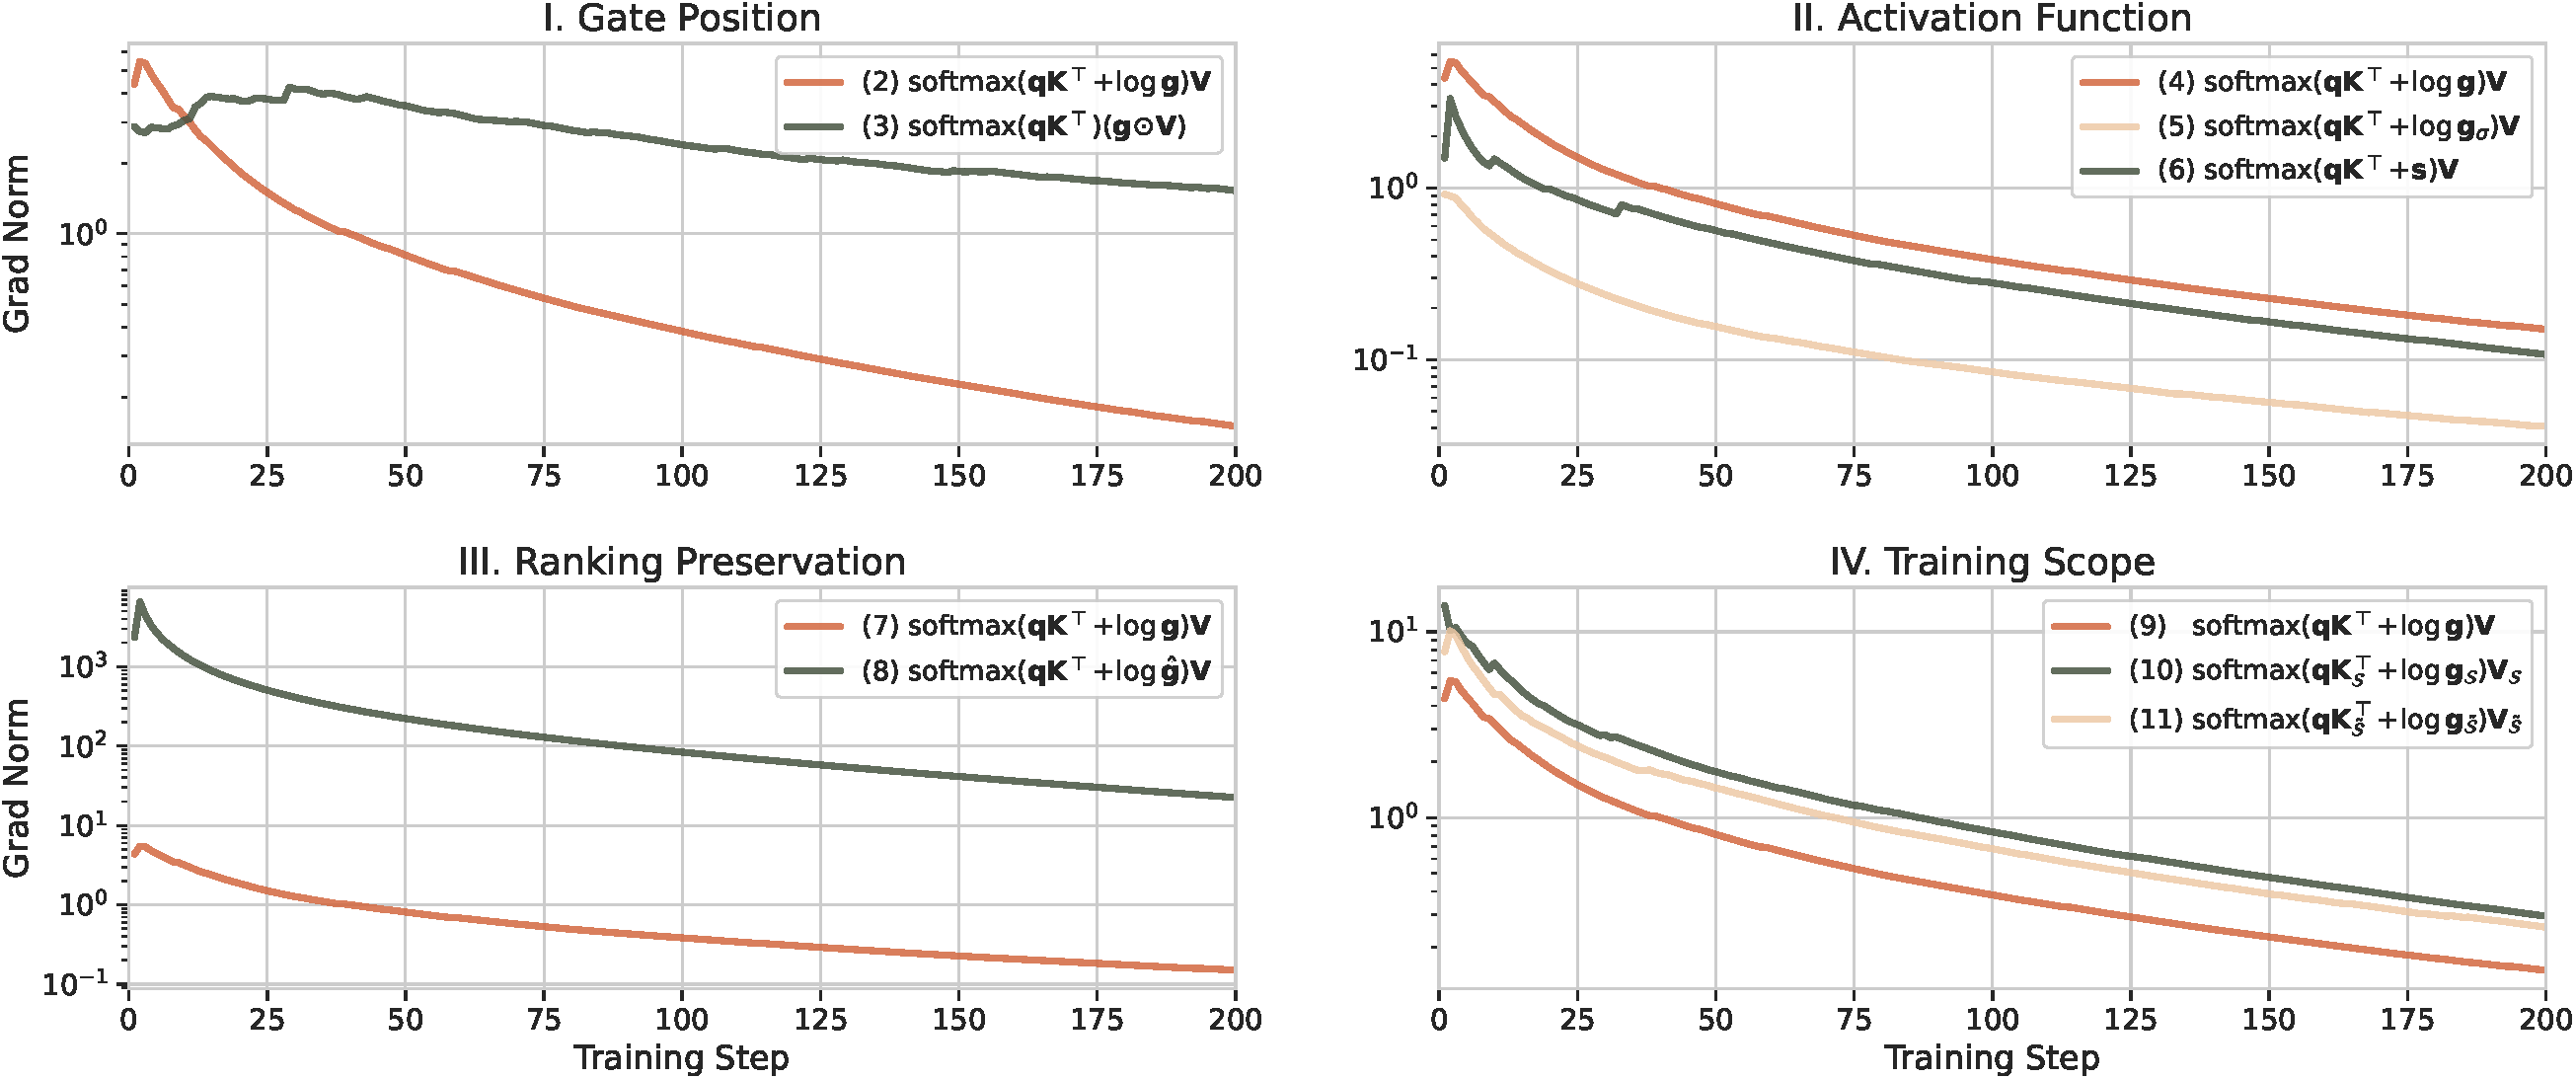
\includegraphics[width=\linewidth]{sec/fig/ablation_gradnorm_curves1.pdf}
        \caption{}
    \end{subfigure}

    \caption{Training dynamics for different gated sparsification designs.
    Inner $\operatorname{softmax}$ gate yields lower training loss than outer gate.
    Independent $\operatorname{sigmoid}$ gates and raw-logit injection achieve lower loss than normalized $\operatorname{softmax}$ gates.
    Hard gating reduces the training loss, but substantially increases the gradient norm.
    Sparse scope training starts with a higher loss but gradually approaches full scope training, while introducing noise yields little difference.}
    \label{fig:loss_ab}
\end{figure}



\section{Limitation}
\label{app:limitation}

We further explore the scalability of the learned selector to RULER \cite{hsieh2024ruler}. Specifically, we sample 0.5B tokens from the \texttt{allenai/dolma3\_longmino\_mix-100B-1125} dataset~\footnote{\url{https://huggingface.co/datasets/allenai/dolma3_longmino_mix-100B-1125}} and train the selector on 64K sequences using a packing strategy. During evaluation, we use the non-thinking mode and extend the context window to 128K with YaRN. As shown in \Cref{tab:ruler}, while \our consistently improves over SeerAttention-R under shorter context lengths, its performance still degrades substantially as the context length increases, leaving a considerable gap from full attention. We believe this limitation primarily stems from the use of pooling based block summaries, which may struggle to preserve fine grained, localized information, such as needle-like signals, within each block, especially as the context length increases. 
Designing more expressive yet efficient selectors that can capture fine-grained information under context block compression is therefore an important direction for future work.

\begin{table}[h]
    \centering
    \caption{
        Evaluation results on the RULER benchmark.
    }
    \label{tab:ruler}
    \resizebox{\textwidth}{!}{
    \begin{tabular}{ll
        rrrrrr
        rrrrrr
        rrrrrr}
    \toprule
    \multirow{2}{*}{\textbf{Budget}} &
    \multirow{2}{*}{\textbf{Method}} &
    \multicolumn{6}{c}{\textbf{Qwen3-4B}} &
    \multicolumn{6}{c}{\textbf{Qwen3-8B}} &
    \multicolumn{6}{c}{\textbf{Qwen3-14B}}
    \\
    \cmidrule(lr){3-8}
    \cmidrule(lr){9-14}
    \cmidrule(lr){15-20}
    &
    &
    \textbf{4K} & \textbf{8K} & \textbf{16K} &
    \textbf{32K} & \textbf{64K} & \textbf{128K}
    &
    \textbf{4K} & \textbf{8K} & \textbf{16K} &
    \textbf{32K} & \textbf{64K} & \textbf{128K}
    &
    \textbf{4K} & \textbf{8K} & \textbf{16K} &
    \textbf{32K} & \textbf{64K} & \textbf{128K}
    \\
    \midrule

    \textit{Full}
    & Full Attn
    & 92.95 & 91.27 & 86.61 & 79.25 & 73.17 & 63.81
    & 93.10 & 90.13 & 89.59 & 87.04 & 77.25 & 73.87
    & 95.28 & 92.71 & 92.91 & 92.15 & 92.19 & 82.23
    \\

    \midrule

    \multirow{2}{*}{2048}
    & SeerAttn-R
    & 92.08 & 79.28 & 56.01 & 30.29 & 18.12 & 13.09
    & 92.15 & 80.16 & 63.76 & 42.16 & 24.49 & 13.99
    & 94.40 & 84.50 & 62.80 & 44.73 & 30.73 & 14.95
    \\
    
    & \our
    & {92.82} & 78.22 & 63.94 & 39.54 & 25.65 & 17.92
    & {92.45} & 81.39 & 69.34 & 46.94 & 30.31 & 19.38
    & 94.43 & 85.10 & 69.01 & 54.76 & 34.12 & 23.80
    \\

    \midrule

    \multirow{2}{*}{4096}
    & SeerAttn-R
    & 93.49 & 87.90 & 72.93 & 47.41 & 27.96 & 16.29
    & 92.96 & 90.13 & 77.39 & 57.92 & 37.43 & 18.75
    & 95.28 & 91.62 & 76.77 & 64.96 & 42.34 & 22.36
    \\

    & \our
    & {93.49} & 89.09 & 75.72 & 51.90 & 35.53 & 21.87
    & {92.96} & 87.96 & 79.88 & 63.50 & 39.18 & 23.46
    & {95.28} & 91.52 & 83.35 & 66.82 & 45.92 & 29.95
    \\

    \bottomrule
    \end{tabular}
    }
\end{table}

\section{Final Performance of Sparse vs.\ Full Training Scope}
\label{app:scope_final}
The gradient analysis in Appendix~\ref{app:deriv_routing_scope} shows that sparse scope updates unselected blocks only indirectly, which slows early optimization but does not change the final ranking quality.
\Cref{tab:scope_final} reports the final accuracy of full scope and sparse scope across Qwen3-4B/8B/14B and token budgets of 1024, 2048, and 4096.
Consistent with the training dynamics in \Cref{tab:ablation_main}, sparse scope matches full scope at convergence across all model scales and budgets, while incurring lower training cost.

\begin{table}[h]
\centering
\caption{Final accuracy (\%) of full training scope versus sparse training scope across model scales and token budgets. Standard deviations are shown in parentheses.}
\label{tab:scope_final}
\resizebox{\textwidth}{!}{
\begin{tabular}{ll lll lll lll lll}
\toprule
\multirow{2}{*}{\textbf{Budget}} & \multirow{2}{*}{\textbf{Train scope}} &
\multicolumn{3}{c}{\textbf{MATH500}} &
\multicolumn{3}{c}{\textbf{GPQA-Diamond}} &
\multicolumn{3}{c}{\textbf{AIME24}} &
\multicolumn{3}{c}{\textbf{AIME25}} \\
\cmidrule(lr){3-5} \cmidrule(lr){6-8} \cmidrule(lr){9-11} \cmidrule(lr){12-14}
& & \textbf{4B} & \textbf{8B} & \textbf{14B}
  & \textbf{4B} & \textbf{8B} & \textbf{14B}
  & \textbf{4B} & \textbf{8B} & \textbf{14B}
  & \textbf{4B} & \textbf{8B} & \textbf{14B} \\
\midrule
\multirow{2}{*}{1024}
& full
& \valstd{91.33}{1.1} & \valstd{91.71}{1.1} & \valstd{93.08}{1.0}
& \valstd{51.42}{2.9} & \valstd{55.62}{2.8} & \valstd{61.77}{2.9}
& - & - & -
& - & - & - \\
& sparse
& \valstd{90.65}{1.1} & \valstd{91.27}{1.1} & \valstd{92.93}{1.0}
& \valstd{50.41}{2.8} & \valstd{53.17}{2.9} & \valstd{61.14}{2.9}
& - & - & -
& - & - & - \\
\midrule
\multirow{2}{*}{2048}
& full
& \valstd{93.00}{1.0} & \valstd{93.09}{1.1} & \valstd{93.56}{1.0}
& \valstd{54.40}{2.9} & \valstd{58.43}{2.9} & \valstd{64.14}{2.8}
& \valstd{68.13}{6.7} & \valstd{70.73}{6.6} & \valstd{76.67}{6.7}
& \valstd{55.39}{7.3} & \valstd{59.27}{7.3} & \valstd{64.04}{7.2} \\
& sparse
& \valstd{93.47}{1.0} & \valstd{93.17}{1.0} & \valstd{93.54}{1.0}
& \valstd{54.86}{2.8} & \valstd{58.74}{2.8} & \valstd{65.09}{2.8}
& \valstd{68.85}{6.6} & \valstd{70.73}{6.7} & \valstd{77.76}{6.6}
& \valstd{56.38}{7.3} & \valstd{58.41}{7.2} & \valstd{64.19}{7.1} \\
\midrule
\multirow{2}{*}{4096}
& full
& \valstd{93.10}{1.0} & \valstd{93.40}{1.0} & \valstd{94.12}{1.0}
& \valstd{54.80}{2.8} & \valstd{60.32}{2.8} & \valstd{64.39}{2.9}
& \valstd{71.17}{6.6} & \valstd{73.52}{6.7} & \valstd{78.49}{6.6}
& \valstd{61.30}{7.3} & \valstd{64.24}{7.1} & \valstd{67.58}{7.0} \\
& sparse
& \valstd{93.67}{1.0} & \valstd{94.23}{1.0} & \valstd{95.23}{0.8}
& \valstd{55.11}{2.9} & \valstd{60.42}{2.8} & \valstd{65.03}{2.8}
& \valstd{71.72}{6.8} & \valstd{73.49}{6.7} & \valstd{78.28}{6.4}
& \valstd{59.97}{7.3} & \valstd{63.41}{7.2} & \valstd{67.29}{6.9} \\
\bottomrule
\end{tabular}
}
\end{table}

\section{Gradient Derivation}
\label{app:derivation}

\subsection{Gradient Derivation for Gate Position}
\label{app:deriv_gate_position}
We derive the gate gradients for outer and inner gate injection.
First, we let
\[
    z_i = \mathbf{q}\mathbf{k}_i^\top,
    \qquad
    p_i = \frac{\exp(z_i)}{\sum_j \exp(z_j)},
    \qquad
    b(i) = m \;\; \text{if } i\in B_m .
\]

\paragraph{Outer gate.}
For outer gating, the attention probability is computed before applying the gate:
\[
    \mathbf{o}_{outer}
    =
    \sum_i p_i g_{b(i)}\mathbf{v}_i .
\]
Since $p_i$ does not depend on $g_m$, the outer-gate gradient is
\[
\begin{aligned}
    dg_m^{outer}
    &=
    \frac{\partial \mathcal{L}}{\partial g_m}
    =
    d\mathbf{o}^{\top}
    \frac{\partial \mathbf{o}_{outer}}{\partial g_m}
    \\
    &=
    d\mathbf{o}^{\top}
    \sum_i
    p_i
    \frac{\partial g_{b(i)}}{\partial g_m}
    \mathbf{v}_i
    \\
    &=
    \sum_{i\in B_m}
    p_i\,
    d\mathbf{o}^{\top}\mathbf{v}_i .
\end{aligned}
\]

\paragraph{Inner gate.}
For inner gating, the gate is injected into the attention logits:
\[
    \mathbf{o}_{inner}
    =
    \sum_i \tilde p_i \mathbf{v}_i,
    \qquad
    \tilde p_i
    =
    \frac{g_{b(i)}\exp(z_i)}
    {\sum_j g_{b(j)}\exp(z_j)} .
\]

For a block gate $g_m$, its derivative is
\[
\begin{aligned}
    \frac{\partial \tilde p_i}{\partial g_m}
    &=
    \frac{
    \mathbb{I}[b(i)=m]\exp(z_i)
    \sum_j g_{b(j)}\exp(z_j)
    -
    g_{b(i)}\exp(z_i)
    \sum_{j\in B_m}\exp(z_j)
    }
    {\left(\sum_j g_{b(j)}\exp(z_j)\right)^2}
    \\
    &=
    \frac{
    \mathbb{I}[b(i)=m]\exp(z_i)
    }
    {\sum_j g_{b(j)}\exp(z_j)}
    -
    \frac{
    g_{b(i)}\exp(z_i)
    }
    {\sum_j g_{b(j)}\exp(z_j)}
    \cdot
    \frac{
    \sum_{j\in B_m}\exp(z_j)
    }
    {\sum_j g_{b(j)}\exp(z_j)}
    \\
    &=
    \frac{\mathbb{I}[b(i)=m]}{g_m}
    \frac{
    g_{b(i)}\exp(z_i)
    }
    {\sum_j g_{b(j)}\exp(z_j)}
    -
    \frac{
    g_{b(i)}\exp(z_i)
    }
    {\sum_j g_{b(j)}\exp(z_j)}
    \cdot
    \sum_{j\in B_m}
    \frac{\exp(z_j)}
    {\sum_r g_{b(r)}\exp(z_r)}
    \\
    &=
    \frac{\mathbb{I}[b(i)=m]}{g_m}\tilde p_i
    -
    \tilde p_i
    \sum_{j\in B_m}
    \frac{1}{g_m}
    \frac{
    g_m\exp(z_j)
    }
    {\sum_r g_{b(r)}\exp(z_r)}
    \\
    &=
    \frac{\mathbb{I}[b(i)=m]}{g_m}\tilde p_i
    -
    \tilde p_i
    \sum_{j\in B_m}
    \frac{\tilde p_j}{g_m}
    \\
    &=
    \tilde p_i
    \left(
        \frac{\mathbb{I}[b(i)=m]}{g_m}
        -
        \sum_{j\in B_m}\frac{\tilde p_j}{g_m}
    \right).
\end{aligned}
\]

Therefore,
\[
\begin{aligned}
    dg_m^{inner}
    &=
    \frac{\partial \mathcal{L}}{\partial g_m}
    =
    d\mathbf{o}^{\top}
    \frac{\partial \mathbf{o}_{inner}}{\partial g_m}
    \\
    &=
    d\mathbf{o}^{\top}
    \sum_i
    \frac{\partial \tilde p_i}{\partial g_m}
    \mathbf{v}_i
    \\
    &=
    d\mathbf{o}^{\top}
    \sum_i
    \tilde p_i
    \left(
        \frac{\mathbb{I}[b(i)=m]}{g_m}
        -
        \sum_{j\in B_m}\frac{\tilde p_j}{g_m}
    \right)
    \mathbf{v}_i
    \\
    &=
    d\mathbf{o}^{\top}
    \left[
    \frac{1}{g_m}
    \sum_{i\in B_m}
    \tilde p_i \mathbf{v}_i
    -
    \frac{1}{g_m}
    \left(
        \sum_{j\in B_m}\tilde p_j
    \right)
    \sum_i \tilde p_i\mathbf{v}_i
    \right]
    \\
    &=
    \frac{1}{g_m}
    d\mathbf{o}^{\top}
    \sum_{i\in B_m}
    \tilde p_i
    \left(
        \mathbf{v}_i-\mathbf{o}_{inner}
    \right)
    \\
    &=
    \sum_{i\in B_m}
    \frac{\tilde p_i}{g_m}
    d\mathbf{o}^{\top}
    \left(
        \mathbf{v}_i-\mathbf{o}_{inner}
    \right).
\end{aligned}
\]


\subsection{Gradient Derivation for Ranking Preservation}
\label{app:deriv_ranking_pres}
Both variants use inner gate injection, so both inherit the inner-gate gradient from Appendix~\ref{app:deriv_gate_position}, with $z_i=\mathbf{q}\mathbf{k}_i^\top$.
They differ only in the attention weight that the forward normalizer assigns to each token.

\paragraph{Soft gating.}
All $C$ blocks stay active, so the normalizer runs over the full context and block $B_m$ appears in its own normalizer:
\[
    \tilde p_i^{soft}
    =
    \frac{g_{b(i)}\exp(z_i)}
    {\sum_j g_{b(j)}\exp(z_j)}
    \le 1,
    \qquad
    dg_m
    =
    \sum_{i\in B_m}
    \frac{\tilde p_i^{soft}}{g_m}\,
    d\mathbf{o}^{\top}
    \left(
        \mathbf{v}_i-\mathbf{o}
    \right).
\]
Hence $\tilde p_i^{soft}\le 1$ for every token, and the gate gradient $dg_m$ stays bounded.

\paragraph{Hard gating with STE.}
The unselected blocks satisfy $\log g^{hard}_m=-\infty$, so the forward normalizer sums only over the selected set $\mathcal{S}=\bigcup_{m\in\mathcal{I}}B_m$.
STE still propagates a gate gradient to a non-selected block $m\notin\mathcal{I}$, whose ranking signal evaluates the attention mass $\tilde p_i^{hard}$ its tokens would receive.
Because $B_m$ is excluded from $\operatorname{LSE}_{\mathcal{S}}$, this weight has no upper bound:
\[
    \tilde p_i^{hard}
    =
    \frac{\exp(z_i)}
    {\sum_{j\in\mathcal{S}}\exp(z_j)}
    =
    \exp\!\left(z_i-\operatorname{LSE}_{\mathcal{S}}\right)
    \le
    \exp\!\left(z_i-\max_{j\in\mathcal{S}}z_j\right),
    \qquad
    \operatorname{LSE}_{\mathcal{S}}
    =
    \log\sum_{j\in\mathcal{S}}\exp(z_j),
\]
which grows exponentially once a dropped block outscores the selected set, $z_i>\max_{j\in\mathcal{S}}z_j$.
The unbounded $\tilde p_i^{hard}$ enters $dg_m$ and, accumulated over all dropped blocks, tokens, and heads, inflates the gate gradient.


\subsection{Gradient Derivation for Training Scope}
\label{app:deriv_routing_scope}
We derive the score gradients under sparse and full scopes.
Let the activation function $\operatorname{softmax}$.

For any gate gradient $dg_\ell$, we first give the $\operatorname{softmax}$ backward formulation
\[
\begin{aligned}
    ds_m
    &=
    \frac{\partial \mathcal{L}}{\partial s_m}
    =
    \sum_{\ell=1}^{C}
    \frac{\partial \mathcal{L}}{\partial g_\ell}
    \frac{\partial g_\ell}{\partial s_m}
    \\
    &=
    \sum_{\ell=1}^{C}
    dg_\ell\,
    g_\ell
    \left(
        \mathbb{I}[\ell=m]-g_m
    \right)
    \\
    &=
    g_m dg_m
    -
    g_m
    \sum_{\ell=1}^{C} g_\ell dg_\ell
    \\
    &=
    g_m
    \left(
        dg_m
        -
        \sum_{\ell=1}^{C} g_\ell dg_\ell
    \right).
\end{aligned}
\]

\paragraph{Sparse routing scope.}
Let $\mathcal{I}=\text{Top-}K(\mathbf{s},K)$ denote the selected block indices.
Under sparse routing scope, only selected blocks participate in the gated attention computation.
For an unselected block $m\notin\mathcal{I}$, the output does not depend on $g_m$, so $dg_m^{sparse}=0$.

Moreover, only selected blocks have nonzero gate gradients:
\[
    dg_\ell^{sparse}=0,
    \qquad
    \ell\notin\mathcal{I}.
\]
Therefore, for $m\notin\mathcal{I}$,
\[
\begin{aligned}
    ds_m^{sparse}
    &=
    g_m
    \left(
        dg_m^{sparse}
        -
        \sum_{\ell=1}^{C}
        g_\ell dg_\ell^{sparse}
    \right)
    \\
    &=
    -g_m
    \sum_{\ell=1}^{C}
    g_\ell dg_\ell^{sparse}
    \\
    &=
    -g_m
    \sum_{\ell\in\mathcal{I}}
    g_\ell dg_\ell^{sparse}.
\end{aligned}
\]

\paragraph{Full routing scope.}
Under full routing scope, all blocks participate in the gated attention computation during training.
Therefore, an unselected block $m\notin\mathcal{I}$ still has its own gate gradient $dg_m^{full}$.
Using the same softmax backward identity,
\[
\begin{aligned}
    ds_m^{full}
    &=
    g_m
    \left(
        dg_m^{full}
        -
        \sum_{\ell=1}^{C}
        g_\ell dg_\ell^{full}
    \right)
    \\
    &=
    -g_m
    \left(
        -dg_m^{full}
        +
        \sum_{\ell=1}^{C}
        g_\ell dg_\ell^{full}
    \right).
\end{aligned}
\]


\definecolor{codeblue}{HTML}{8A8A8A}
\definecolor{codekw}{HTML}{CB7C5E}
\definecolor{codesign}{HTML}{A5432D}
\definecolor{codefunc}{HTML}{D1917F}


\lstdefinelanguage{PythonFuncColor}{
  language=Python,
  keywordstyle=\color{codesign}\bfseries,
  commentstyle=\color{codeblue},  %
  stringstyle=\color{orange},
  showstringspaces=false,
  basicstyle=\ttfamily\small,
  literate=
    {*}{{\color{codesign}* }}{1}
    {dataloader}{{\color{codefunc}dataloader}}{1}
    {sample_t_r}{{\color{codefunc}sample\_t\_r}}{1}
    {randn}{{\color{codefunc}randn}}{1}
    {randn_like}{{\color{codefunc}randn\_like}}{1}
    {jvp}{{\color{codefunc}jvp}}{1}
    {stopgrad}{{\color{codefunc}stopgrad}}{1}
    {metric}{{\color{codefunc}metric}}{1}
}

\lstset{
  language=PythonFuncColor,
  backgroundcolor=\color{white},
  basicstyle=\fontsize{9pt}{9.9pt}\ttfamily\selectfont,
  columns=fullflexible,
  breaklines=true,
  captionpos=b,
  frame=none
}


\section{Kernel Implementation}
\label{sec:app_kernel}

We provide a custom Triton implementation for the sparse scope soft gated attention used during SAS training.
The block gate is organized as a table $\log\mathbf{G}$, where each query position and attention head holds one log gate value for every previous context block.
Block selection is encoded by a per query threshold $\tau$: a block is \emph{selected} when its log gate reaches the threshold ($\log g_m\ge\tau$), which realizes the Top-$K$ set $\mathcal{I}$ without an explicit sort. Non selected blocks are masked out of the softmax so that only the selected set $\mathcal{S}$ participates.

For simplicity of presentation, the pseudocode omits the grouped query attention, and variable length packing that the full implementation supports, and focuses on the gate injection and the sparse scope.

\paragraph{Forward pass.}
The kernel traverses causal key value blocks in a tiled manner.
The current (self) block always uses a unit gate and a causal mask, so local causal attention is always preserved.
For each earlier block, the kernel maps key positions to their block index, loads the corresponding log gate, and adds it to the $\mathbf{q}\mathbf{K}_{\mathcal{S}}^\top$ scores before the online softmax update; blocks below the threshold are masked to $-\infty$ and an entire block is skipped when no query in the tile selects it.

\paragraph{Backward pass.}
We follow the standard recomputation based attention backward procedure.
The kernel first computes the row-wise correction term $\mathbf{\Delta}=\sum_d\mathbf{O}_d\cdot d\mathbf{O}_d$.
It then recomputes the gated attention probabilities from the saved log-sum-exp values and uses them to obtain gradients for $\mathbf{Q}$, $\mathbf{K}$, and $\mathbf{V}$.
In addition, the gradient of each block log gate is accumulated by summing the score gradients over all tokens inside the corresponding selected block, producing a compact block-level gradient tensor that is propagated back to the selector.
As a result, the implementation supports sparse scope gated attention training without storing the dense attention matrix.

\begin{algorithm}
\caption{Forward Pass of Fused SAS Kernel}
\label{alg:soft_gate_fwd}
\begin{lstlisting}[language=python]
def gated_scores(q, k, logG, tau, q_tile, kv_tile, B, sm_scale, self_block):
    S = sm_scale * matmul(q, k.T)
    b = block_id(kv_tile, B)
    if self_block:
        # current block: unit gate (log 1 = 0), causal mask
        return apply_causal_mask(S, q_tile, kv_tile)
    log_g = load(logG, q_tile, b)               # [q_rows] per-query block gate
    active = log_g >= load(tau, q_tile)         # selected blocks only (Top-K set)
    S = S + broadcast(log_g, kv_tile)           # inject gate inside softmax
    return where(active, S, -inf)               # mask out non-selected blocks

def soft_gate_fwd(Q, K, V, logG, tau, B, sm_scale):
    O, LSE = empty_output(Q, V), empty_lse(Q)

    for q_tile in tiles(Q):
        q = load(Q, q_tile)
        m, l = full(q.rows, -inf), zeros(q.rows)
        acc = zeros(q.rows, V.dim)

        # Phase 1: self block (causal) ; Phase 2: earlier blocks (sparse)
        for kv_tile in causal_tiles(K, q_tile):
            self_block = in_self_block(kv_tile, q_tile, B)
            if (not self_block) and no_query_selects(logG, tau, q_tile, kv_tile, B):
                continue                        # skip fully non-selected block
            k, v = load(K, kv_tile), load(V, kv_tile)
            S = gated_scores(q, k, logG, tau, q_tile, kv_tile, B, sm_scale, self_block)

            m_new = maximum(m, rowmax(S))
            P = exp(S - m_new[:, None])
            acc = acc * exp(m - m_new)[:, None] + matmul(P, v)
            l = l * exp(m - m_new) + rowsum(P)
            m = m_new

        O[q_tile] = acc / l[:, None]
        LSE[q_tile] = m + log(l)

    return O, LSE
\end{lstlisting}
\end{algorithm}

\begin{algorithm}
\caption{Backward Pass of Fused SAS Kernel}
\label{alg:soft_gate_bwd}
\begin{lstlisting}[language=python]
def soft_gate_bwd(Q, K, V, logG, tau, O, dO, LSE, B, sm_scale):
    dQ, dK, dV = zeros_like(Q), zeros_like(K), zeros_like(V)
    dLogG, Delta = zeros_like(logG), rowsum(O * dO)

    # ---- Pass 1: dQ and dLogG (loop q outer, kv inner) ----
    for q_tile in tiles(Q):
        q, do = load(Q, q_tile), load(dO, q_tile)
        lse, delta = load(LSE, q_tile), load(Delta, q_tile)
        dq = zeros_like(q)

        for kv_tile in causal_tiles(K, q_tile):
            self_block = in_self_block(kv_tile, q_tile, B)
            if (not self_block) and no_query_selects(logG, tau, q_tile, kv_tile, B):
                continue
            k, v = load(K, kv_tile), load(V, kv_tile)
            S = gated_scores(q, k, logG, tau, q_tile, kv_tile, B, sm_scale, self_block)

            P = exp(S - lse[:, None])
            dS = P * (matmul(do, v.T) - delta[:, None])
            dq += sm_scale * matmul(dS, k)
            if not self_block:
                for b in blocks(kv_tile, B):
                    # gate gradient: sum dS over kv tokens in the selected block
                    dLogG[q_tile, b] += rowsum(dS[:, tokens(kv_tile, b)])

        dQ[q_tile] = dq

    # ---- Pass 2: dK and dV (loop kv outer, q inner) ----
    for kv_tile in tiles(K):
        k, v = load(K, kv_tile), load(V, kv_tile)
        dk, dv = zeros_like(k), zeros_like(v)

        for q_tile in attending_q_tiles(Q, kv_tile):
            self_block = in_self_block(kv_tile, q_tile, B)
            if (not self_block) and no_query_selects(logG, tau, q_tile, kv_tile, B):
                continue
            q, do = load(Q, q_tile), load(dO, q_tile)
            lse, delta = load(LSE, q_tile), load(Delta, q_tile)
            S = gated_scores(q, k, logG, tau, q_tile, kv_tile, B, sm_scale, self_block)

            P = exp(S - lse[:, None])
            dS = P * (matmul(do, v.T) - delta[:, None])
            dk += sm_scale * matmul(dS.T, q)
            dv += matmul(P.T, do)

        dK[kv_tile], dV[kv_tile] = dk, dv

    return dQ, dK, dV, dLogG
\end{lstlisting}
\end{algorithm}


